\feelchapter{Natural convection in a heated tank}
            {Natural convection in a heated tank}
            {Christophe Prud'homme}
            {cha:natural-convection-2d}

\newcommand{\Gr}{\ensuremath{\mathrm{Gr}\xspace}}
\renewcommand{\Pr}{\ensuremath{\mathrm{Pr}\xspace}}

\section{Description}
\label{sec:description}

The goal of this project is to simulate the fluid flow under natural
convection: the heated fluid circulates towards the low temperature
under the action of density and gravity differences. Thie phenomenon
is important in the sense it models evacuation of heat, generated by
friction forces for example, with  a cooling fluid.

We shall put in place a simple convection problem in order to study
the phenomenon without having to handle the difficulties of more
complex domaines. We describe then some necessary transformations to
the equations, then we define quantities of interest to be able to
compare the simulations with different parameter values.


\newcommand{\Water}{\text{\textsc{Water}}\xspace}
\newcommand{\Fluid}{\text{\textsc{Fluid}}\xspace}
\tikzstyle{snakearrow} = [decoration={snake,aspect=0.2,segment length=1cm,amplitude=1mm},decorate]

\begin{figure}[htbp]
  \centering
  \begin{tikzpicture}[thick,scale=5]

    %% draw axis
    \draw[->] (-0.6,-0.4) -- (1.1,-0.4) node[right] {$x$} coordinate (x axis);
    \draw[-] (-0.,-0.39) -- (0,-0.41) node[below] {$0$};
    \draw[-] (1.,-0.39) -- (1,-0.41) node[below] {$W$};
    \draw[->] (-0.4,-0.6) -- (-0.4,1.1) node[above] {$y$} coordinate (y axis);
    \draw[-] (-0.39,-0.) -- (-0.41,-0.) node[left] {$0$};
    \draw[-] (-0.39,1.) -- (-0.41,1) node[left] {$1$};

    %% draw top and down walls
    \fill[pattern={north east lines},pattern color=blue] (0,1) rectangle  (1,1.02) ;
    \fill[pattern={north west lines},pattern color=blue] (0,0) rectangle  (1,-0.02) ;

    %% Draw the domain
    \draw[very thick,fill=blue!10!white,draw=blue!50] (0,0) rectangle  (1,1) ;
    \node at (0.1,0.5) {$\Gamma_1$};
    \node at (0.5,0.1) {$\Gamma_2$};
    \node at (0.9,0.5)  {$\Gamma_3$};
    \node at (0.8,0.9)  {$\Gamma_4$};
    \node (omega) at (0.5,0.3)  {$\Omega (\Fluid)$};
    % \draw[->,snakearrow] (omega) -- (0.5,0.5);
    \draw[<->] (0,-0.1) -- (1,-0.1) node [below,midway] {$W$};
    \draw[-] (0.5,1.) -- (0.5,0.5) node[left,midway] {$\Gamma_f$};
    \draw[-,ultra thick,color=blue] (0,0) -- (0,1) node [left,midway] {$T_0$};
    \draw[-,ultra thick,color=red] (1,0) -- (1,1)  {};


    \foreach \y in {0.1,0.3,0.5,0.7,0.9} {
      %%\draw[->] (\x, -1.5) -- (\x,\pgfmathqparse{-0.7*\x*\x+0.7*8*\x-12} \pgfmathresult);
      %%\pgfmathsetmacro{\pgf@x}{\x}
      %%\pgfmathparse{-0.7*\pgf@x*\pgf@x+0.7*8*\pgf@x-0.7*12}
      %%\def\y{\pgfmathresult}
      \def\x{1.3}
      \draw[->] (1.3, \y) -- (1.1,\y);
    }
    \node at (1.6,0.5) {Heat flux};

  \end{tikzpicture}
  \caption{Geometry of the model}
  \label{fig:heatns:1}
\end{figure}

To study the convection, we use a model problem: it consists in a
rectangular tank of height $1$ and width $W$, in which the fluid is
enclosed, see figure~\ref{fig:heatns:1}. We wish to know the fluid velocity
$\mathbf{u}$, the fluid pressure $p$ and fluid temperature $\theta$.

We introduce the adimensionalized Navier-Stokes and heat equations
parametrized by the Grashof and Prandtl numbers. These parameters
allow to describe the various regimes of the fluid flow and heat
transfer in the tank when varying them.

The adimensionalized steady incompressible Navier-Stokes equations reads:
\begin{equation}
  \label{eq:38}
  \begin{split}
    \mathbf{u}\cdot\nabla \mathbf{u} +\nabla p -\frac{1}{\sqrt{\Gr}} \Delta \mathbf{u} &= \theta \mathbf{e}_2\\
    \nabla \cdot \mathbf{u} & = 0\ \text{sur}\ \Omega\\
    \mathbf{u} & = \mathbf{0}\ \text{sur}\ \partial \Omega
  \end{split}
\end{equation}
where $\Gr$ is the Grashof number, $\mathbf{u}$ the adimensionalized
velocity and $p$ adimensionalized pressure and $\theta$ the
adimensionalized temperature. The temperature is in fact the
difference between the temperature in the tank and the temperature
$T_0$ on boundary $\Gamma_1$.

The heat equation reads:
\begin{equation}
  \label{eq:37}
  \begin{split}
    \mathbf{u} \cdot \nabla \theta -\frac{1}{\sqrt{\Gr}\Pr} \Delta \theta &= 0\\
    \theta &= 0\ \text{sur}\ \Gamma_1\\
    \frac{\partial \theta}{\partial n} &= 0\ \text{sur}\ \Gamma_{2,4}\\
    \frac{\partial \theta}{\partial n} &= 1\ \text{sur}\ \Gamma_3
  \end{split}
\end{equation}
where $\Pr$ is the Prandtl number.

% \section{Nombre de Grashof}
% \label{sec:nombre-de-grashof}
% Le nombre de Grashof (\Gr) est un nombre sans dimension utilisé en
% mécanique des fluides pour caractériser la convection libre dans un
% fluide. Il correspond au rapport des forces de gravité sur les forces
% visqueuses.

% On le définit de la manière suivante
% \begin{equation}
%   \label{eq:18}
%   \Gr = \frac{g\  \beta\  (T-T_\infty)\  {L_c}^3}{\nu^2}
% \end{equation}
% avec:
% \begin{itemize}
% \item $g$ - constante gravitationnelle
% \item $\beta$ - coefficient de dilatation
% \item $T-T_\infty$ - différence de température
% \item $L_c$ - longueur caractéristique
% \item $\nu$ - viscosité cinématique
% \end{itemize}

% \section{Nombre de Prandtl}
% \label{sec:nombre-de-prandtl}

% Le nombre de Prandtl (\Pr) est un nombre sans dimension. Il représente
% le rapport entre la diffusivité de quantité de mouvement $\nu$ (ou
% viscosité cinématique) et la diffusivité thermique.

% On le définit de la manière suivante
% \begin{equation}
%   \label{eq:19}
%   \Pr=\frac {\mu C_p }{\lambda}=\frac {\mu}{\frac {k}{C_p}}=\frac {\frac {\mu}{\rho}}{\frac {k}{\rho C_p}}=\frac {\nu}{\alpha}
% \end{equation}
% avec
% \begin{itemize}
% \item $\nu$ la viscosité cinématique en $m^2\cdot s^{-1}$
% \item $\rho$ la masse volumique en $kg\cdot m^{-3}$
% \item $\alpha$ la diffusivité thermique en $m^2\cdot s^{-1}$
% \item $\mu$ la viscosité dynamique en $N\cdot s\cdot m^{-2}$
% \item $C_p$ la chaleur massique en $J\cdot kg^{-1}\cdot K^{-1}$
% \item $k$ la conductivité thermique $W \cdot m^{-1}\cdot K^{-1}$
% \end{itemize}



\section{Influence of parameters}
\label{sec:infl-des-param}


what are the effects of the Grashof and Prandtl numbers ? We remark
that both terms with these parameters appear in front of the $\Delta$
parameter, they thus act on the diffusive terms. If we increase the
Grashof number or the Prandtl number the coefficients multiplying the
diffusive terms decrease, and this the convection, that is to say the
transport of the heat via the fluid, becomes dominant. This leads also
to a more difficult and complex flows to simulate, see
figure~\ref{fig:heatns:2}. The influence of the Grashof and Prandtl
numbers are different but they generate similar difficulties and flow
configurations. Thus we look only here at the influence of the Grashof
number which shall vary in $[1, 1e7]$.

\begin{figure}[htbp]
  \centering
  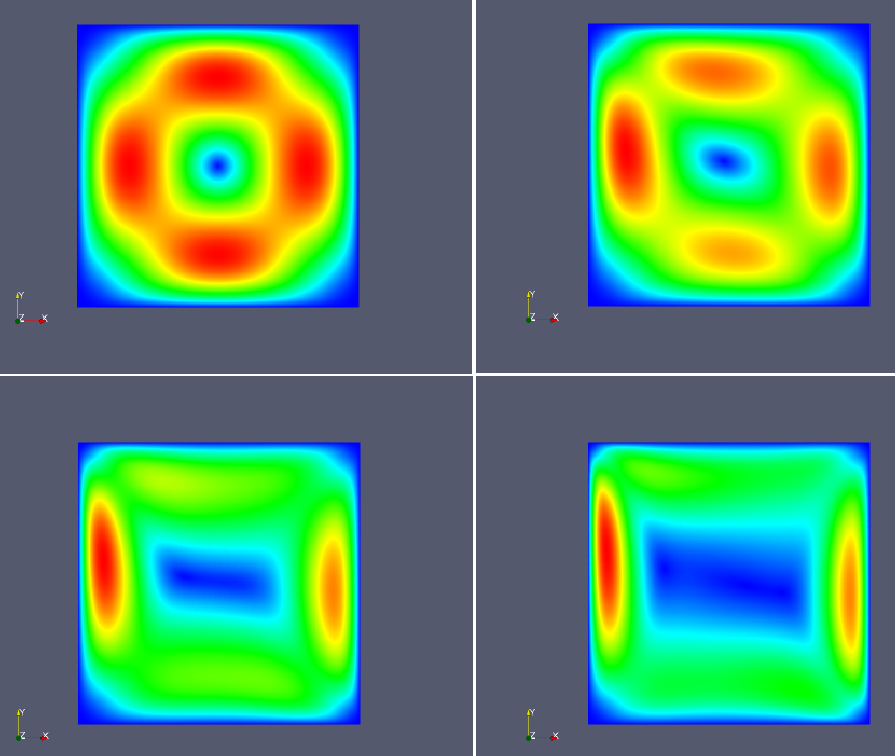
\includegraphics[width=.8\linewidth]{pngs/flow_grashof}
  \caption{Velocity norm with respect to  Grashof, $\Gr=100, 10000,
    100000, 500000$. $h=0.01$ and $\Pr=1$.}
  \label{fig:heatns:2}
\end{figure}

\section{Quantities of interest}
\label{sec:quant-du-benchm}

We would like to compare the results of many simulations with respect
to the Grashof defined in the previous section. We introduce two
quantities which will allow us to observe the behavior of the flow and
heat transfer.


\subsection{Mean temperature}
\label{sec:mean-temperature}

We consider first the mean temperature on boundary $\Gamma_3$
\begin{equation}
  \label{eq:16}
  T_3 = \int_{\Gamma_3} \theta
\end{equation}

This quantity should decrease with increasing Grashof because the
fluid flows faster and will transport more heat which will cool down
the heated boundary $\Gamma_3$. We observe this behavior on the
figure~\ref{fig:heatns:3}.

\begin{figure}[htbp]
  \centering
  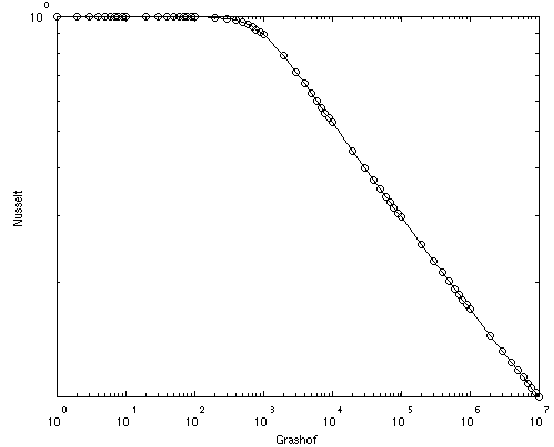
\includegraphics[width=.8\linewidth]{pngs/temp_grashof}
  \caption{Mean temperature with respect to the Grashof number;
    $h=0.02$ with $\mathbb{P}_3$ Lagrange element for the velocity,
    $\mathbb{P}_2$ Lagrange for the pressure and $\mathbb{P}_1$
    Lagrange for the temperature.}
  \label{fig:heatns:3}
\end{figure}

\subsection{Flow rate}
\label{sec:flow-rate}

Another quantity of interest is the flow rate through the middle of the
tank. We define a segment $\Gamma_f$ as being the vertical top
semi-segment located at $W/2$ with height $1/2$, see
figure~\ref{fig:heatns:1}. The flow rate, denoted $\mathrm{D}_f$, reads
\begin{equation}
  \label{eq:17}
  \mathrm{D}_f =  \int_{\Gamma_f} \mathbf{u} \cdot \mathbf{e}_1
\end{equation}
where $\mathbf{e}_1=(1,0)$. Note that the flow rate can be negative or
positive depending on the direction in which the fluid flows.

As a function of the Grashof, we shall see a increase in the flow
rate. This is true for small Grashof, but starting at $1e3$ the flow
rate decreases. The fluid is contained in a boundary layer which is
becoming smaller as the Grashof increases.

\begin{figure}[htbp]
  \centering
  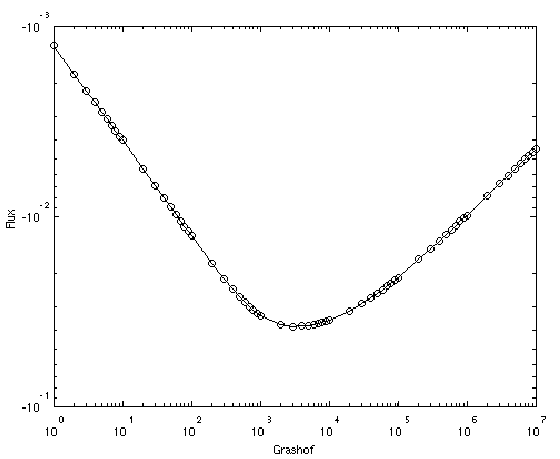
\includegraphics[width=.8\linewidth]{pngs/debit_grashof}
  \caption{Behavior of the flow rate with respect to the Grashof number; $h = 0.02$,
    $\mathbb{P}_3$ for the velocity, $\mathbb{P}_2$ for the pressure and
    $\mathbb{P}_1$ for the temperature.}
  \label{fig:4}
\end{figure}

\section{Implementation}
\label{sec:implementation}

This application in implemented in
\texttt{life/doc/tutorial/convection*.cpp}. The implementation solve
the full nonlinear problem using the nonlinear solver framework.

\section{Numerical Schemes}
\label{sec:numerical-schemes}

\subsection{Stokes problem formulation and the pressure}
\label{sec:stok-probl-form}

\subsection{The Stokes problem}
\label{sec:stokes-problem}

Consider the following problem,
\begin{equation}
  \label{notes:eq:16}
  \mbox{Stokes: }\left\{
    \begin{array}{rcc}
      -\mu\Delta\mathbf{u} +
      \nabla p =
      \mathbf{f}\\
      \nabla\cdot\mathbf{u} = 0\\
      \mathbf{u}|_{\partial \Omega} = 0
    \end{array}
  \right.
\end{equation}
where $\Omega \subset \mathbb{R}^d$. There are no boundary condition
on the pressure. This problem is ill-posed, indeed we only control the
pressure through its gradient $\nabla p$. Thus if $(\mathbf{u},p)$ is
a solution, then $(\mathbf{u},p+c)$ is also a solution with $c$ any
constant. This comes from the way the problem is posed: the box is
closed and it is not possible to determine the pressure inside. The
remedy is to impose arbitrarily a constraint on the pressure, e.g. its
mean value is zero. In other words, we add this new equation to the
problem (\ref{notes:eq:16})
\begin{equation}
  \label{notes:eq:17}
  \int_\Omega p = 0
\end{equation}
\begin{remark}[The Navier-Stokes case]
  This is also true for the incompressible Navier-Stokes equations. We
  chose Stokes to simplify the exposure.
\end{remark}

\subsection{Reformulation}
  In order to impose the condition~(\ref{notes:eq:17}), we introduce a new
  unknown, a Lagrange multiplier, $\lambda \in \mathbb{R}$ and modify
  the incompressibility equation. Our problem reads now, find
  $(\mathbf{u},p,\lambda)$ such
  that
    \begin{equation}
      \label{notes:eq:18}
    \mbox{Stokes 2: }\left\{
      \begin{array}{rcl}
        -\mu\Delta\mathbf{u} +
        \nabla p &=&
        \mathbf{f}\\
        \nabla\cdot\mathbf{u} + \lambda &=& 0\\
        \mathbf{u}|_{\partial \Omega} &=& 0\\
        \int_\Omega p &=& 0
      \end{array}
    \right.
\end{equation}
\begin{remark}[The pressure as Lagrange multiplier]
  The pressure field $p$ can actually be seen as a Lagrange multiplier
  for the velocity $\mathbf{u}$ in order to enforce the constraint
  $\nabla \cdot \mathbf{u} = 0$. $\lambda$ will play the same role but
  for the pressure to enforce the condition (\ref{notes:eq:17}). As $h
  \rightarrow 0$, $\lambda \rightarrow 0$ as well as the divergence of
  $\mathbf{u}$. Note also that $\int_\Omega \nabla \cdot \mathbf{u}
  \approx - \int_\Omega \lambda$ from the second equation.
\end{remark}

\subsection{Variational formulation}
\label{sec:vari-form}

The variational formulation now reads: find $(\mathbf{u}, p,
\lambda) \in \mathbf{H}^1_0(\Omega) \times L^2_0(\Omega) \times
\mathbb{R}$ such that for all $(\mathbf{v}, q, \eta) \in
\mathbf{H}^1_0(\Omega) \times L^2_0(\Omega) \times \mathbb{R}$

\begin{equation}
  \label{notes:eq:20}
  \mbox{Stokes 3: }\left\{
    \begin{array}{rcl}
      \int_\Omega \Big(\nabla \mathbf{u} \colon \nabla \mathbf{v} + \nabla \cdot \mathbf{v} p\Big) &=& \int_\Omega \mathbf{f} \cdot \mathbf{v}\\
      \int_\Omega \Big(\nabla\cdot\mathbf{u} q + \lambda q\Big)   &=& 0\\
      \int_\Omega p \eta &=& 0
    \end{array}
  \right.
\end{equation}

Summing up all three equations we get the following condensed formulation:

\begin{equation}
  \label{notes:eq:19}
  \int_\Omega \nabla \mathbf{u} \colon \nabla \mathbf{v} + \nabla \cdot \mathbf{v} p + \nabla \cdot \mathbf{u} q + \lambda q + \eta p = \int_\Omega \mathbf{f} \cdot \mathbf{v}
\end{equation}
where $\mathbf{H}^1_0(\Omega)= \Big\{ \mathbf{v} \in \mathbf{L}^2(\Omega), \nabla \mathbf{v} \in [L^2(\Omega)]^{d\times d},\ \mathbf{v} = 0\ \text{on}\ \partial \Omega \Big\}$,
$L^2_0(\Omega)= \Big\{ v \in L^2(\Omega),\ \int_\Omega v = 0\Big\}$, and
$\mathbf{L}^2(\Omega)= \Big\{ \mathbf{v} \in [L^2(\Omega)]^d\Big\}$ that is to say each component of a  vector field of $\mathbf{L}^2(\Omega)$ are in $L^2(\Omega)$.


\subsection{Implementation}
\label{sec:implementation}

  \begin{lstlisting}
/*basis*/
typedef Lagrange<Order, Vectorial> basis_u_type; // velocity
typedef Lagrange<Order-1, Scalar> basis_p_type; // pressure
typedef Lagrange<0, Scalar> basis_l_type; // multipliers
typedef bases<basis_u_type, basis_p_type, basis_l_type> basis_type;
/*space: product of the velocity, pressure and multiplier spaces*/
typedef FunctionSpace<mesh_type, basis_type, value_type> space_type;
// ...
space_ptrtype Xh = space_type::New( mesh );
element_type U( Xh, "u" );
element_type V( Xh, "v" );
element_0_type u = U.element<0>();
element_0_type v = V.element<0>();
element_1_type p = U.element<1>();
element_1_type q = V.element<1>();
element_2_type lambda = U.element<2>();
element_2_type nu = V.element<2>();
// ...
sparse_matrix_ptrtype D( M_backend->newMatrix( Xh, Xh ) );
form2( Xh, Xh, D, _init=true )=
   integrate( elements(mesh), im,
             // $\nabla \mathbf{u} \colon \nabla \mathbf{v}$
              mu*trace(deft*trans(def))
              // $\nabla \cdot \mathbf{v} p + \nabla \cdot \mathbf{u} q$
              - div(v)*idt(p) + divt(u)*id(q)
              // $\lambda q + \eta p$
              +id(q)*idt(lambda) + idt(p)*id(nu) );
// ...
  \end{lstlisting}


\subsection{Fix point iteration for Navier-Stokes}
\label{sec:fix-point-iteration}

\subsubsection{Steady incompressible Navier-Stokes equations}
  Consider the following steady incompressible Navier-Stokes
  equations, find $(\mathbf{u},p)$ such that
  \begin{equation}
    \label{notes:eq:7}
    \begin{split}
      \underbrace{\rho \mathbf{u} \cdot \nabla \mathbf{u}}_{\text{convection}} - \underbrace{\nu \Delta  \mathbf{u}}_{\text{diffusion}} + \nabla p &=  \mathbf{f} \ \text{on}\ \Omega \\
      \nabla \cdot \mathbf{u} &= 0 \\
      \mathbf{u} &= \mathbf{0}\ \text{on}\ \partial \Omega
    \end{split}
  \end{equation}
  where $\rho$ is the density of the fluid, $\nu$ is the dynamic
  viscosity of the fluid(la viscosité cinématique $\eta = \nu/\rho$) and $\mathbf{f}$ is the external force
  density applied to the fluid, (e.g. $\mathbf{f}=-\rho g \mathbf{e}_2$ with $\mathbf{e}_2=(0,1)^T$ ).  This equation system is nonlinear due
  to the $\mathbf{u} \cdot \nabla \mathbf{u}$ convection term. A
  simple approach to solve~(\ref{notes:eq:7}) is to use a fix point
  algorithm.


The fixpoint algorithm for NS reads as follows, find
$(\mathbf{u}^{(k)},p^{(k)})$ such that
    \begin{equation}
      \label{notes:eq:13}
    \begin{split}
      \rho\mathbf{u}^{(k-1)} \cdot \nabla \mathbf{u}^{(k)} - \nu \Delta  \mathbf{u}^{(k)} + \nabla p^{(k)} &= \mathbf{f} \ \text{on}\ \Omega \\
      \nabla \cdot \mathbf{u}^{(k)} &= 0 \\
      \mathbf{u}^{(k)} &= 0\ \text{on}\ \partial \Omega\\
      (\mathbf{u}^{(0)},p^{(0)}) &= (\mathbf{0},0)
    \end{split}
  \end{equation}
  The system~(\ref{notes:eq:13}) is now linear at each iteration $k$ and we
  can write the variational formulation accordingly. A stopping
  criterium is for example that
  $\|\mathbf{u}^{k}-\mathbf{u}^{(k-1)}\|+\|p^{k}-p^{(k-1)}\| <
  \epsilon$ where $\epsilon$ is a given tolerance (e.g. $1e-4$) and
  $\|\cdot\|$ is the $L_2$ norm.

  Here is the implementation using \Feel:

  \begin{lstlisting}
    // define some tolerance $\epsilon$
    epsilon = 1e-4;
    // set $(\mathbf{u}^{(0)},p^{(0)})$ to $(\mathbf{0},0)$
    velocity_element_type uk(Xh);
    velocity_element_type uk1(Xh);
    pressure_element_type pk(Ph);
    pressure_element_type pk1(Ph);
    // by default uk1, uk and pk,pk1 are initialized to 0

    // assemble the linear form associated to $\mathbf{f}$
    // store in vector $F$, it does not change over the iterations

    // iterations to find $(\mathbf{u}^{(k)},p^{(k)})$
    do
    {
      // save results of previous iterations
      uk1 = uk;
      pk1 = pk;

      //assemble for bilinear form  associated to
      // $\rho\mathbf{u}^{(k-1)} \cdot \nabla \mathbf{u}^{(k)} - \nu \Delta  \mathbf{u}^{(k)} + \nabla p^{(k)}$
      // store in matrix $A^{(k)}$

      // solve the system $A^{(k)} X = F$ where $X = (\mathbf{u}^{(k)},p^{(k)})^T$

      // use uk,uk1 and pk,pk1 to compute the error estimation at each iteration
      error = $\|\mathbf{u}^{k}-\mathbf{u}^{(k-1)}\|+\|p^{k}-p^{(k-1)}\|$
    } while( error > epsilon );

  \end{lstlisting}

\subsection{A Fix point coupling algorithm}
\label{sec:coupling-algorithm}

\subsubsection{Coupling fluid flow and heat transfer: problem}
  Recall that we have to solve two coupled problems :

  $$
  \mbox{Heat(\textbf{u}) }\left\{
  \begin{array}{rcc}
    - \kappa\Delta T + \mathbf{u}\cdot\nabla T &=& 0 \\
    T|_{\Gamma_1} &=& T_0 \\
    \frac{\partial T}{\partial \mathbf{n}}|_{\Gamma_3} &=&1 \\
    \frac{\partial T}{\partial \mathbf{n}}|_{\Gamma_2,\Gamma_4} &=& 0
  \end{array}
  \right.
  $$

  and

  $$\mbox{Stokes(T) : }\left\{
    \begin{array}{rcc}
      -\nu\Delta\mathbf{u} +
      \frac{1}{\rho}\nabla p =
      \mathbf{F}\\
      \nabla\cdot\mathbf{u} = 0\\
      \mathbf{u}|_{\partial \Omega} = 0
    \end{array}
  \right.
  $$

Where $\mathbf{F}$ can be taken as $
 \left(
  \begin{array}{c}
    0 \\
    \beta(T-T_0)
  \end{array}
\right)
$
for some $\beta > 0$. $\beta$ is called the \emph{dilatation coefficient}.

\subsubsection{Coupling fluid flow and heat transfer: algorithm}
Here is a simple algorithm fix point strategy in pseudo-code:
\begin{lstlisting}
   double tol = 1.e-6;
   int maxIter = 50;
   //Initial guess Un = 0
   do
   {
     // Find Tn solution of Heat(Un)
     // Find Unp1 solution of Stokes(Tn)
     // compute stopTest = norme(Unp1 - Un)
     // Un = Unp1
   }while((stopTest < tol) && (niter <= maxIter));
\end{lstlisting}

\begin{remark}[The unsteady case]
  To solve the unsteady problems, one can insert the previous loop in
  the one dedicated to time discretization
\end{remark}

\subsection{A Newton coupling algorithm}
\label{sec:newt-coupl-algor}

\subsubsection{A fully coupled scheme}

  Another possiblity is to use a Newton method which allows us to
  solve the full nonlinear problem coupling velocity, pressure and
  temperature
  \begin{equation}
    \label{notes:eq:21}
    \text{Find}\ X\ \text{such that}\ F(X) = 0
  \end{equation}
  the method is iterative and reads, find $X^{(n+1)}$ such that
  \begin{equation}
    \label{notes:eq:22}
    J_F(X^{(n)})( X^{(n+1)}-X^{(n)}) = - F (X^{(n)})
  \end{equation}
  starting with $X^{(0)} = \mathbf{0}$ or some other initial value and
  where $J_F$ is the jacobian matrix of $F$ evaluated at
  $X=((u_i)_i,(p_i)_i,(\theta_i)_i)^T$.  For any $\phi_k, \psi_l$ and
  $\rho_m$ the \emph{test} functions associated respectively to velocity,
  pressure and temperature, our full system reads, Find $X=((u_i)_i,(p_i)_i,(\theta_i)_i)^T$ such that
  \begin{equation}
    \label{notes:eq:23}
    \begin{array}{rll}
      F_1((u_i)_i,(p_i)_i,(\theta_i)_i)&=\sum_{i,j} u_i u_j a(\phi_i,\phi_k,\phi_j) - \sum_i p_i b(\phi_k,\psi_i) + \sum_i \theta_i c(\rho_i, \phi_k)+\sum_i u_i d(\phi_i,\phi_k)  &= 0\\
      F_2((u_i)_i,(p_i)_i,(\theta_i)_i)&=\sum_i u_i b(\phi_i,\psi_l) &=0\\
      F_3((u_i)_i,(p_i)_i,(\theta_i)_i)&=\sum_{i,j} u_i\theta_j e(\phi_i,\rho_j,\rho_m) + \sum_i \theta_i f(\rho_i,\rho_m)-g(\rho_m) &=  0
    \end{array}
  \end{equation}
  where $F=(F_1,F_2,F_3)^T$ and
  \begin{equation}
    \label{notes:eq:26}
    \begin{array}{rl}
    a(\mathbf{u},\mathbf{v},\beta) &= \int_\Omega \mathbf{v}^T ((\nabla \mathbf{u} )\beta)\\
    b(\mathbf{v},p) &= \int_\Omega p (\nabla \cdot \mathbf{v}) - \int_{\partial \Omega} \mathbf{v}\cdot\mathbf{n} p\\
      c(\theta,\mathbf{v})&= \int_\Omega \theta \mathbf{e}_2 \cdot \mathbf{v}\\
      d(\mathbf{u},\mathbf{v}) &= \frac{1}{\sqrt{\mathrm{Gr}}} \Big(\int_\Omega \nabla \mathbf{u} \colon (\nabla \mathbf{v})^T - \int_{\partial \Omega} ((\nabla \mathbf{u}) \mathbf{n})\cdot \mathbf{v}\Big)\\
      e(\mathbf{u},\theta,\chi) &= \int_\Omega (\mathbf{u}\cdot \nabla \theta) \chi \\
      f(\theta,\chi) &=\frac{1}{\sqrt{\mathrm{Gr}}\mathrm{Pr}} \Big( \int_\Omega \nabla \theta \cdot \nabla \chi - \int_{\Gamma_1} (\nabla \theta \cdot \mathbf{n} ) \chi \Big)\\
      g(\chi) &=\frac{1}{\sqrt{\mathrm{Gr}}\mathrm{Pr}} \int_{\Gamma_3} \chi
    \end{array}
  \end{equation}
  \begin{remark}
    Note that the boundary integrals are kept in order to apply the
    weak Dirichlet boundary condition trick, see next section~\ref{sec:weak-dirichl-boud}.
  \end{remark}

\subsubsection{Jacobian matrix}
  In order to apply the newton scheme, we need to compute the jacobian
  matrix $J_F$ by deriving each equation with respect to each
  unknowns, ie $u_i, p_i$ and $\theta_i$.
  Consider the first equation
  \begin{itemize}
  \item Deriving the first equation with respect to $u_i$ we get
    \begin{equation}
      \label{notes:eq:30}
      \frac{\partial F_1}{\partial u_i} = \sum_j u_j a(\phi_i,\phi_k,\phi_j) + \sum_i u_i a(\phi_i,\phi_k,\phi_j) + d(\phi_i,\phi_k)
    \end{equation}
  \item Deriving the first equation with respect to $p_i$ we get
    \begin{equation}
      \label{notes:eq:30}
      \frac{\partial F_1}{\partial p_i} =  -b(\phi_k,\psi_l)
    \end{equation}
  \item Deriving the first equation with respect to $\theta_i$ we get
    \begin{equation}
      \label{notes:eq:30}
      \frac{\partial F_1}{\partial \theta_i} = c(\rho_i,\rho_k)
    \end{equation}

  \end{itemize}
  Consider the second equation, only the derivative with respect to $u_i$ is non zero.
  \begin{equation}
    \label{notes:eq:31}
    \frac{\partial F_2}{\partial u_i} = b(\phi_i,\psi_l)
  \end{equation}
  Finally the third component
  \begin{itemize}
  \item Deriving with respect to $u_i$
    \begin{equation}
      \label{notes:eq:33}
      \frac{\partial F_3}{\partial u_i} = \sum_j \theta_j e(\phi_i,\rho_j,\rho_m)
    \end{equation}
  \item Deriving with respect to $p_i$,
    \begin{equation}
      \label{notes:eq:34}
      \frac{\partial F_3}{\partial p_i} = 0
    \end{equation}
  \item Deriving with respect to $theta_i$,
    \begin{equation}
      \label{notes:eq:35}
      \frac{\partial F_3}{\partial \theta_i} = \sum_j u_j e(\phi_j,\rho_i,\rho_m) + f(\rho_i,\rho_m)
    \end{equation}
  \end{itemize}
  \begin{equation}
    \label{notes:eq:35}
    J_F =
    \begin{pmatrix}
      \frac{\partial F_1}{\partial u_i} & \frac{\partial F_1}{\partial p_i} & \frac{\partial F_1}{\partial \theta_i} \\
      {\frac{\partial F_2}{\partial u_i}} & {\frac{\partial F_2}{\partial p_i}}(=0) & {\frac{\partial F_2}{\partial \theta_i}}(=0) \\
      \frac{\partial F_3}{\partial u_i} & {\frac{\partial F_3}{\partial p_i}}(=0) & \frac{\partial F_3}{\partial \theta_i}
    \end{pmatrix}
  \end{equation}
  In order to implement $J_F$ and solve (\ref{notes:eq:22}), $J_F$ can be
  expressed as the matrix associated with the discretisation of
  \begin{equation}
    \label{notes:eq:37}
    \begin{array}{rl}
      a(\mathbf{u},\mathbf{v},\beta_1) + a(\beta_1, \mathbf{v}, \mathbf{u})+d(\mathbf{u},\mathbf{v})-b(\mathbf{v},p)+c(\theta,\mathbf{v}) &= 0\\
      b(\mathbf{u},q)&=0\\
      e(\beta_1,\theta,\chi)+f(\theta,\chi)+e(\mathbf{u},\beta_2,\chi)&=0\\
    \end{array}
  \end{equation}
  where $\beta_1 = u^{(n)}$, $\beta_2=\theta^{(n)}$ are known from the
  previous Newton iteration, indeed $J_F$ is actually evaluated in $X^{(n)}$.

\subsubsection{\Feel Implementation}
  Now we use the \Feel non linear framework in order to implement our
  Newton scheme~(\ref{notes:eq:22}).
  We need to define two new functions in our application
  \begin{itemize}
  \item \texttt{updateJacobian(X,J)} which takes as input \texttt{X}$=X^{(n)}$ and returns the matrix \texttt{J=}$J_F(X^{(n)})$
  \item \texttt{updateResidual(X,R)} which takes as input \texttt{X}$=X^{(n)}$ and returns the vector \texttt{R=}$F(X^{(n)})$
  \end{itemize}

  \begin{remark}{Backend}
    Only the PETSC backend supports the nonlinear solver framework.
    Use  in the command line like in the first section
    \begin{lstlisting}
      --backend=petsc
    \end{lstlisting}
  \end{remark}

  Here is a snippet of code that implements the nonlinear framework.
  \begin{lstlisting}
    class MyApp
    {
      public:
      void run();
      void updateResidual( const vector_ptrtype& X, vector_ptrtype& R );
      void updateJacobian( const vector_ptrtype& X, sparse_matrix_ptrtype& J);
      void solve( sparse_matrix_ptrtype& D, element_type& u, vector_ptrtype& F );
      private:

      backend_ptrtype M_backend;
      sparse_matrix_ptrtype M_jac;
      vector_ptrtype M_residual;
    };

    void
    MyApp::run()
    {
      // ...

      // plug the updateResidual and updateJacobian functions
      // in the nonlinear framework
      M_backend->nlSolver()->residual = boost::bind( &self_type::updateResidual,
                                                     boost::ref( *this ), _1, _2 );
      M_backend->nlSolver()->jacobian = boost::bind( &self_type::updateJacobian,
                                                     boost::ref( *this ), _1, _2 );

      vector_ptrtype U( M_backend->newVector( u.functionSpace() ) );
      *U = u;
      vector_ptrtype R( M_backend->newVector( u.functionSpace() ) );
      this->updateResidual( U, R );
      sparse_matrix_ptrtype J;
      this->updateJacobian( U, J );
      solve( J, u, R );

      *U = u;
      this->updateResidual( U, R );
      // R(u) should be small
      std::cout << "R( u ) = " << M_backend->dot( U, R ) << "\n";


    }
    void
    MyApp::solve( sparse_matrix_ptrtype& D, element_type& u, vector_ptrtype& F )
    {
      vector_ptrtype U( M_backend->newVector( u.functionSpace() ) );
      *U = u;
      M_backend->nlSolve( D, U, F, 1e-10, 10 );
      u = *U;
    }
    void
    MyApp::updateResidual( const vector_ptrtype& X, vector_ptrtype& R )
    {
      // compute R(X)

      R=M_residual;
    }
    void
    MyApp::updateJacobian( const vector_ptrtype& X, vector_ptrtype& R )
    {
      // compute J(X)

      J=M_jac;
    }
  \end{lstlisting}
  see \texttt{bratu.cpp} or \texttt{nonlinearpow.cpp} for example.


%%% Local Variables:
%%% coding: utf-8
%%% mode: latex
%%% TeX-PDF-mode: t
%%% TeX-parse-self: t
%%% x-symbol-8bits: nil
%%% TeX-auto-regexp-list: TeX-auto-full-regexp-list
%%% TeX-master: "../feel-manual"
%%% ispell-local-dictionary: "american"
%%% End:

